\subsection{Inner tracker}
\label{sec:tracker}

The purpose of the inner tracker of the CMS detector
is to precisely and efficiently measure the trajectories
of charged particles produced by LHC collisions.
Reconstructed particle trajectories are known as ``tracks''.
The inner tracker is composed of about 200~$m^2$ of active silicon area, 
making it the largest silicon tracker ever built.
It rests within the bore of the 
CMS solenoid (Section \ref{sec:solenoid}), which
provides a homogenous magnetic field of 3.8 T around
the full inner tracker volume.  
By reconstructing trajectories of charged particles with 
$\pt > 1$~\GeV, the inner tracker fulfills several important tasks.
First, the inner tracker makes it possible to reconstruct primary decay vertices,
secondary decay vertices, and the displacement of tracks from those 
vertices (known as the track ``impact parameter''), which allow
for the identification of heavy flavor quarks.
Second, along with the electromagnetic calorimeter (Section \ref{sec:ecal}) and 
the muon system (Section \ref{sec:muon}), the inner tracker allows for the identification
of electrons and muons.  Third,
the inner tracker allows for the identification of tau leptons by identifying various decay topologies.
In addition, the inner tracker provides essential input to the high level trigger (Section \ref{sec:trigger}).
As shown in the schematic cross section in Figure \ref{fig:tracker}, the inner tracker is made up of two
detector subsystems: the pixel tracker and the strip tracker.  Both detectors the cover
pseudorapidity region $|\eta| < 2.5$.  The resolution of several track parameters is shown in Figure
\ref{fig:tracker-resolution}.

\begin{figure}
  \centering
  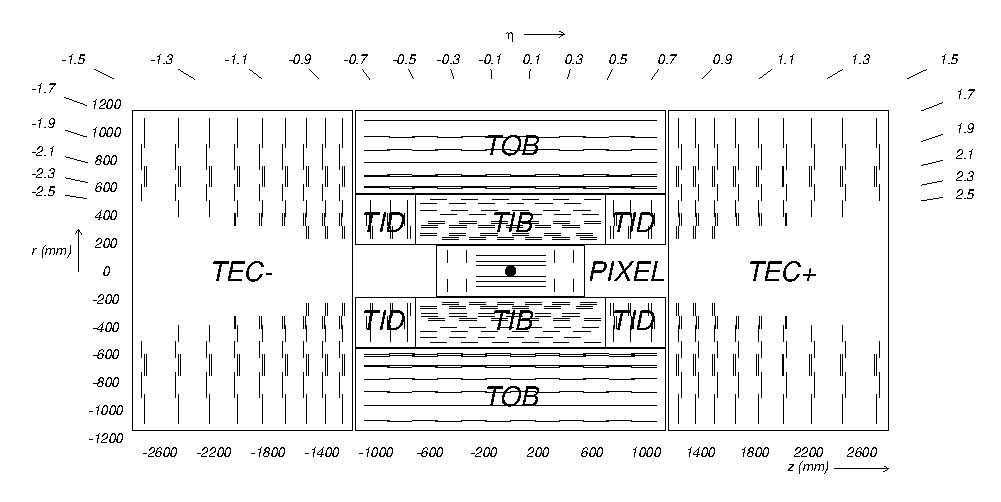
\includegraphics[width=0.95\textwidth]{tex/cms/fig/tracker-schematic.pdf}
  \caption{A schematic cross section of the inner tracker of the CMS detector.  The pixel tracker
    is labeled near the interaction point at the center of the schematic.
    The four components of the silicon strip tracker (TIB, TOB, TID, and TEC) are also shown  \cite{cms-jinst}.}
  \label{fig:tracker}
\end{figure}

\begin{figure}
  \centering
  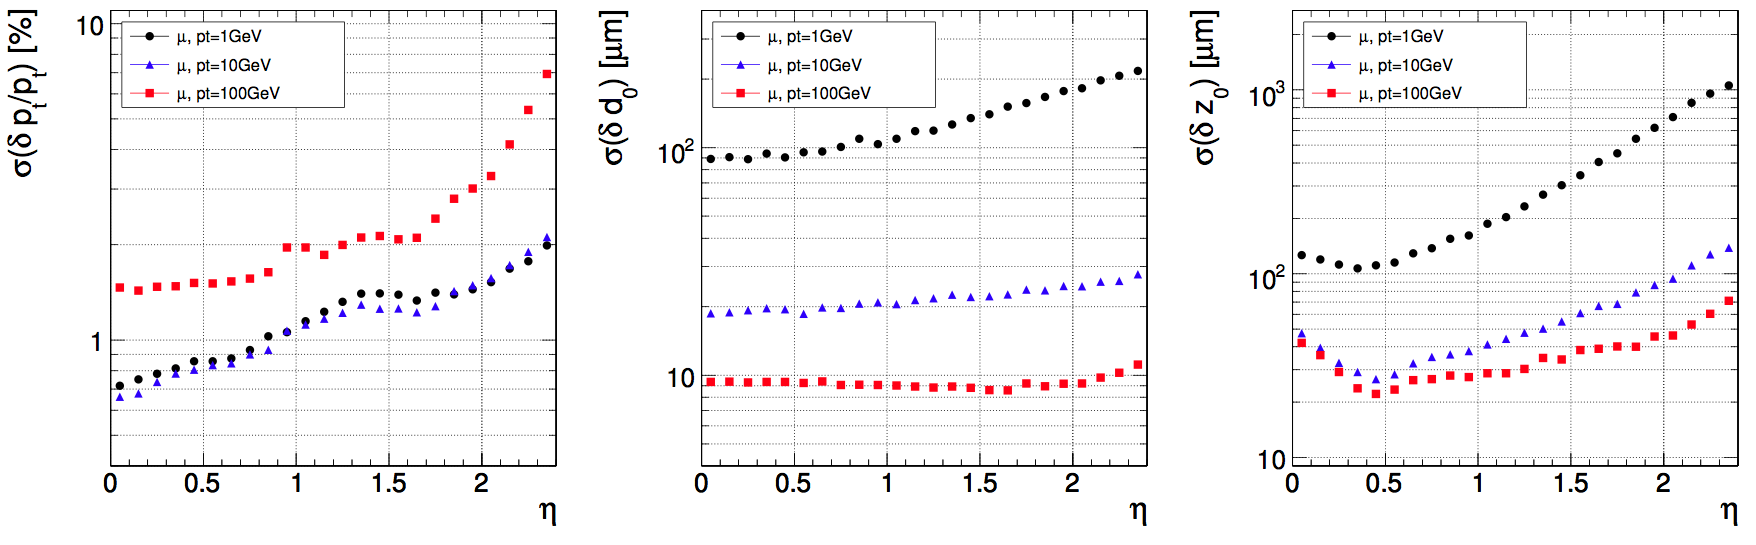
\includegraphics[width=0.95\textwidth]{tex/cms/fig/tracker-resolution.png}
  \caption{The resolution of various parameters of muon tracks as a function of the absolute value of 
    pseudorapidity as reconstructed by the CMS inner tracker.  The plot on the left shows transverse momentum,
    the central plot shows transverse impact parameter, and the plot on the right shows
    longitudinal impact parameter.  Black markers correspond to muons with a transverse momentum of 1 GeV,
    blue markers correspond to muons with a transverse momentum of 10 GeV, and 
    red markers correspond to muons with a transverse momentum of 100 GeV \cite{cms-jinst}.}
  \label{fig:tracker-resolution}
\end{figure}

The pixel detector consists of three barrel layers (BPix)
\nomenclature{BPix}{Barrel pixel detector}
and two endcap disks (FPix) on either side of the IP.  
\nomenclature{FPix}{Forward pixel detector}
The BPix layers are 53 cm long and have mean radii of 4.4, 7.3, and 10.2 cm.  
The FPix layers extend from 6 to 15 cm in radius and are 
placed on either size at $z = \pm 34.5$ cm and $z = \pm 46.6$ cm.
A schematic is shown in Figure \ref{fig:pixel}.
The pixel detector consists of 66 million pixel cells in total 
(48 million in BPix, 18 million in FPix).  Each pixel is 
$100 \times 150$~$\mu\text{m}^2$, and the total active silicon area for the pixel detector
is 1.06~$\text{m}^2$ (0.78~$\text{m}^2$ in BPix and 0.28~$\text{m}^2$
in FPix).  Pixels of this size are chosen to ensure an occupancy of $10^{-4}$ per LHC crossing
at design beam energy and instantaneous luminosity.
Even during heavy ion collisions, this occupancy is about $10^{-2}$ in the pixel detector, allowing for
efficiency track reconstruction in a high particle density environment.
This arrangement of the FPix and BPix detectors ensures that
the pixel detector offers three hit coverage over nearly the entire
pseudorapidity range. 

\begin{figure}
  \centering
  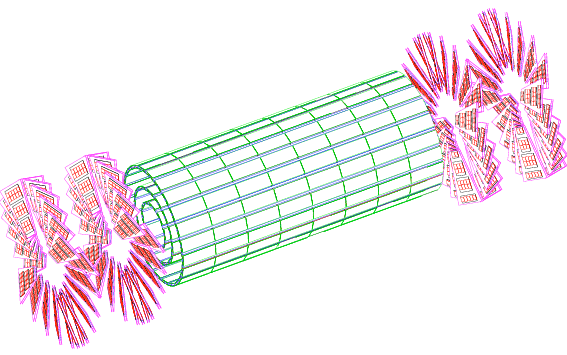
\includegraphics[width=0.8\textwidth]{tex/cms/fig/tracker-pixel-schematic.png}
  \caption{A schematic of the pixel tracker of the CMS detector.  
    The three barrel layers (BPix) are shown in green. The four 
    endcap disks (FPix) are shown in pink \cite{cms-tdr}.}
  \label{fig:pixel}
\end{figure}

The strip detector surrounds the pixel detector in the radial
region between 20 and 116 cm, and it is made up of four separate 
detector subsystems.
The inner barrel region of the strip detector extends in radius out to 
55 cm and is made up of four barrel layers (TIB)
\nomenclature{TIB}{Tracker inner barrel}
with three disks at each end (TID).
\nomenclature{TIB}{Tracker inner disk}
In this region, the particle 
flux is low enough to allow the use of silicon microstrip 
detectors with minimum cell size of 10 cm $\times$ 80 $\mu\text{m}$, while
still maintaining an occupancy of 2-3\% per $pp$ LHC crossing at
design beam energy and instantaneous luminosity.
The outer barrel region of the strip detector extends in radius from 55 cm to 116 cm
and is made up of an additional 6 barrel layers (TOB)
\nomenclature{TOB}{Tracker outer barrel}.
In this region, the particle flux is lower still, which allows the use
of larger-pitch silicon microstrips with a maximum cell size of 25 cm $\times$ 
180 $\mu\text{m}$, while still maintaining an occupancy of 1\% per $pp$ LHC crossing at
design beam energy and instantaneous luminosity.
The TIB, TID, and TOB subsystems collectively extend in out to 
$z=\pm 118$~cm.  Beyond this $z$ range are 9 additional disks on either side (TEC), 
\nomenclature{TEC}{Tracker endcap} 
occupying the region 124 cm $< |z| <$ 282 cm and 22.5 cm $< |r| < $ 113.5 cm.
The first two layers in both the TIB and TOB subsystems, 
the first two disks of the TID subsystem, and disks 1, 2, and 5 of the TEC subsystem 
are made with modules
that are laid in stereo in order to provide a measurement in both $r-\phi$ and $r-z$ 
coordinates.  
The pixel detector consists of 9.3 million silicon microstrips in total, and the
total active silicon area for the strip detector is 198 $\text{m}^2$.
This layout makes it likely that each track has at least nine hits in the region $|\eta| < 2.4$
with at least four two-dimensional measurements.

The CMS inner tracker operates in a high flux of particles, which
can cause radiation damage both to the front-end electronics and to 
the silicon itself.  In order to minimize this radiation damage and 
to ensure a high track finding efficiency and a low fake rate, 
the CMS tracker is operated at a temperature of $-10\,^{\circ}{\rm C}$.
This is made more difficult by two effects:  first, the detector itself
disappates nearly 60 kW of power; and second, the tracker faces the
electromagnetic calorimeter, which must be operated at room temperature and must have good temperature stability.
These effeets are overcome by lining the interior of the tracker's support structure
with an active, 32-panel thermal screen.  On the inside of the screen, cold fluid is
circulated in a thin aluminum plate to keep the tracker cool.  On the other 
side of 8mm of Rohacell foam, insulated resistive circuits are powered to keep the outer
surface warm enough to avoid condensation.  The screen acts in concert with the
individual cooling systems of the inner tracker subsystems.  It  ensures a temperature
below $-10\,^{\circ}{\rm C}$ inside the tracker volume and a temperature of 
$+12\,^{\circ}{\rm C}$ outside the tracker support structure, even when the 
inner tracker subsystems and their cooling systems are shut off.
\cite{cms-jinst,cms-tdr}.
